\documentclass[11pt]{article}
\usepackage[margin=1in]{geometry}
\usepackage{amsmath,amssymb,amsthm}
\usepackage{graphicx}
\usepackage{tikz}
\usetikzlibrary{decorations.pathreplacing} % <-- FIX: Required for the braces in Q4
\usepackage{enumitem}
\usepackage{hyperref}

\newtheorem{proposition}{Proposition}
\newcommand{\Z}{\mathbb{Z}}
\newcommand{\N}{\mathbb{N}}

\title{Problem Set 2 --- Answer Key\\\large Origins of Mathematics, Fall 2026}
\author{}
\date{}

\begin{document}
	\maketitle
	
	\noindent\textbf{Grading note.} A proof must justify the general case; numerical examples alone earn no credit for ``prove'' parts. Diagrams must be labeled.
	
	%==========================================================
	\section{Squaring numbers ending in 5}
	
	\subsection*{(a) Conjecture}
	If $n$ is a positive integer whose decimal representation ends in 5, write $n = 10k+5$ with $k \ge 0$. Then
	\[
	n^2 = 100\,k(k+1) + 25.
	\]
	In words: \emph{delete the final 5, multiply the remaining number by the next integer, and append 25.}
	
	\subsection*{(b) Four examples}
	\[
	55^2 = 3025,\quad 65^2 = 4225,\quad 75^2 = 5625,\quad 85^2 = 7225.
	\]
	(Check: $5\cdot 6=30$, $6\cdot 7=42$, $7\cdot 8=56$, $8\cdot 9=72$, each followed by 25.)
	
	\subsection*{(c) Proof}
	Let $n = 10k+5$. Then
	\[
	n^2 = (10k+5)^2 = 100k^2 + 100k + 25 = 100\,k(k+1) + 25.
	\]
	Since $k(k+1)$ is an integer, $100\,k(k+1)$ occupies the decimal places from the hundreds upward, and the added $25$ occupies exactly the tens and units places. Hence the decimal representation of $n^2$ is the decimal representation of $k(k+1)$ followed by the two digits ``25.'' (When $k=0$, $n=5$ and $n^2=25$, consistent with the empty prefix.) \qed
	
	%==========================================================
	\section{Finding a pair}
	
	Partition $\{1,2,\dots,8\}$ into the four pairs
	\[
	\{1,8\},\quad \{2,7\},\quad \{3,6\},\quad \{4,5\},
	\]
	each of which sums to $9$.
	
	\subsection*{(a) Proof}
	Choosing five distinct numbers from a set partitioned into four pairs means, by the \textbf{Pigeonhole Principle}, that two of the chosen numbers lie in the same pair. Any two members of a pair $\{j, 9-j\}$ sum to $9$. Hence some two chosen numbers add to $9$. \qed
	
	\subsection*{(b) Four numbers with no pair summing to 9}
	Yes. Example: $\{1,2,3,4\}$. No two of these sum to $9$ (the largest possible sum is $3+4=7$). More generally, choosing at most one element from each of the four pairs yields a valid set of size $4$; e.g.\ $\{1,2,3,4\}$, $\{1,2,3,5\}$, $\{1,2,6,7\}$, etc.
	
	\emph{Sharpness.} Four is the maximum: by part (a), any five numbers force a pair summing to $9$.
	
	%==========================================================
	\section{A remainder problem}
	
	We seek the smallest $n \in \N$ with
	\[
	n \equiv 1 \pmod 2,\qquad n \equiv 4 \pmod 5,\qquad n \equiv 8 \pmod{11}.
	\]
	The moduli $2,5,11$ are pairwise coprime, so the Chinese Remainder Theorem guarantees a unique solution modulo $M = 2\cdot 5\cdot 11 = 110$.
	
	\subsection*{(a) Sun Zi reconstruction}
	
	\textbf{Step 1 (unit contributions).} For each modulus $m_i$, set $M_i = M/m_i$ and find $y_i$ with $M_i y_i \equiv 1 \pmod{m_i}$:
	\[
	\begin{aligned}
		m_1=2:&\quad M_1 = 55, & 55y_1 \equiv 1 \pmod 2 &\iff y_1 \equiv 1 \pmod 2, & y_1 &= 1.\\
		m_2=5:&\quad M_2 = 22, & 22y_2 \equiv 1 \pmod 5 &\iff 2y_2 \equiv 1 \pmod 5, & y_2 &= 3.\\
		m_3=11:&\quad M_3 = 10, & 10y_3 \equiv 1 \pmod{11} &\iff -y_3 \equiv 1 \pmod{11}, & y_3 &= 10.
	\end{aligned}
	\]
	(Check: $55\cdot 1 = 55 \equiv 1 \pmod 2$; $22\cdot 3 = 66 \equiv 1 \pmod 5$; $10\cdot 10 = 100 \equiv 1 \pmod{11}$.)
	
	\textbf{Step 2 (combine with remainders).} The reconstruction formula gives
	\[
	n \equiv \sum_i r_i M_i y_i \pmod M
	= 1\cdot(55\cdot 1) + 4\cdot(22\cdot 3) + 8\cdot(10\cdot 10) \pmod{110}.
	\]
	Compute:
	\[
	55 + 4\cdot 66 + 8\cdot 100 = 55 + 264 + 800 = 1119.
	\]
	Reduce modulo $110$:
	\[
	1119 = 10\cdot 110 + 19 \implies n \equiv 19 \pmod{110}.
	\]
	The smallest positive solution is $\boxed{n = 19}$.
	
	\subsection*{(b) Verification}
	\[
	19 = 2\cdot 9 + 1 \;\checkmark,\qquad
	19 = 5\cdot 3 + 4 \;\checkmark,\qquad
	19 = 11\cdot 1 + 8 \;\checkmark.
	\]
	
	\subsection*{(c) All solutions}
	Since the moduli are pairwise coprime, CRT gives a unique residue class modulo $110$. Hence the full solution set is
	\[
	\boxed{n = 19 + 110t,\quad t = 0,1,2,\dots}
	\]
	\emph{Why this is complete:} if $n$ and $n'$ are two solutions, then $n - n'$ is divisible by each of $2, 5, 11$, hence by their product $110$ (coprimality). So any two solutions differ by a multiple of $110$, and every number of the form $19 + 110t$ satisfies all three congruences. \qed
	
	%==========================================================
	\section{Trisecting a line segment}
	
	\subsection*{(a) Construction}
	Given segment $AB$.
	
	\begin{enumerate}[label=\textbf{Step \arabic*.}]
		\item Draw a ray $\ell$ from $A$ at any convenient angle to $AB$ (not collinear with $AB$).
		\item With compass set to any convenient radius $r$, strike off three equal segments along $\ell$ from $A$: obtain points $P_1, P_2, P_3$ with
		\[
		AP_1 = P_1P_2 = P_2P_3 = r.
		\]
		\item Draw line $P_3B$.
		\item Through $P_1$ and $P_2$, construct lines parallel to $P_3B$ (copy the angle $\angle AP_3B$ at $P_1$ and $P_2$; Euclid I.23/I.31).
		\item Let the parallel through $P_1$ meet $AB$ at $T_1$, and the parallel through $P_2$ meet $AB$ at $T_2$.
	\end{enumerate}
	
	\noindent\textbf{Result:} $T_1, T_2$ trisect $AB$.
	
	\begin{center}
		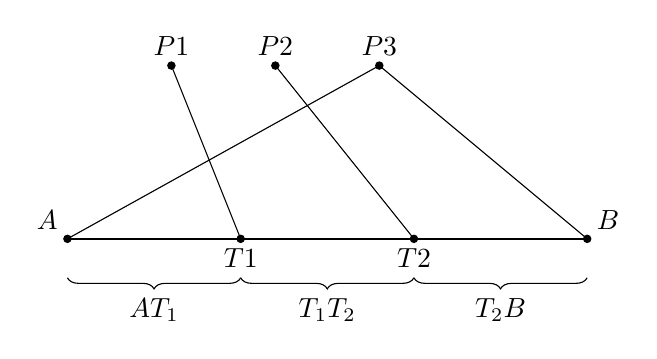
\begin{tikzpicture}[scale=1.1]
			\coordinate (A) at (0,0);
			\coordinate (B) at (6,0);
			\coordinate (P1) at (1.2,2.0);
			\coordinate (P2) at (2.4,2.0);
			\coordinate (P3) at (3.6,2.0);
			\coordinate (T1) at (2,0);
			\coordinate (T2) at (4,0);
			\draw[thick] (A)--(B);
			\draw (A)--(P3);
			\draw (P3)--(B);
			\draw (P1)--(T1);
			\draw (P2)--(T2);
			\foreach \p/\l in {A/above left, B/above right, P1/above, P2/above, P3/above, T1/below, T2/below}
			\fill (\p) circle (1.4pt) node[\l] {$\p$};
			\draw[decorate,decoration={brace,amplitude=4pt,mirror}] (0,-0.45)--(2,-0.45) node[midway,below=4pt]{$AT_1$};
			\draw[decorate,decoration={brace,amplitude=4pt,mirror}] (2,-0.45)--(4,-0.45) node[midway,below=4pt]{$T_1T_2$};
			\draw[decorate,decoration={brace,amplitude=4pt,mirror}] (4,-0.45)--(6,-0.45) node[midway,below=4pt]{$T_2B$};
		\end{tikzpicture}
	\end{center}
	
	\subsection*{(b) Proof}
	Apply \textbf{Euclid VI.2} to triangle $AP_3B$. Since $P_1T_1 \parallel P_3B$,
	\[
	\frac{AT_1}{T_1P_3} = \frac{AP_1}{P_1P_3} = \frac{r}{2r} = \frac12.
	\]
	Equivalently, $AT_1 : T_1B = 1:2$ in triangle $ABP_3$ with $P_1T_1 \parallel P_3B$, so $AT_1 = \tfrac13 AB$.
	
	Similarly, $P_2T_2 \parallel P_3B$ gives $AT_2 : T_2B = AP_2 : P_2P_3 = 2r : r = 2:1$, so $AT_2 = \tfrac23 AB$.
	
	Therefore
	\[
	T_1T_2 = AT_2 - AT_1 = \tfrac23 AB - \tfrac13 AB = \tfrac13 AB,
	\]
	and $T_2B = AB - AT_2 = \tfrac13 AB$. Hence
	\[
	AT_1 = T_1T_2 = T_2B = \tfrac13 AB. \qed
	\]
	
	\subsection*{Optional extension}
	To divide $AB$ into $n$ equal parts: lay off $n$ equal segments $AP_1 = P_1P_2 = \cdots = P_{n-1}P_n$ along the auxiliary ray, draw $P_nB$, and through each $P_i$ ($1 \le i \le n-1$) draw the parallel to $P_nB$. By VI.2, the intersections on $AB$ cut it in the ratio $1:1:\cdots:1$, i.e.\ into $n$ equal parts.
	
	%==========================================================
	\section{One quadratic, three methods}
	
	Equation: $\;x^2 + 10x = 39$.
	
	\subsection*{(a) Geometry (four-rectangle completion)}
	
	Begin with a square of side $x$ (area $x^2$). The term $10x$ is represented by four congruent rectangles, one attached to each side of the square. Since $10x = 4\cdot(2.5x)$, each rectangle has dimensions
	\[
	x \times \tfrac{10}{4} = x \times 2.5,
	\]
	so each has area $2.5x$, and the four together have area $10x$.
	
	\begin{center}
		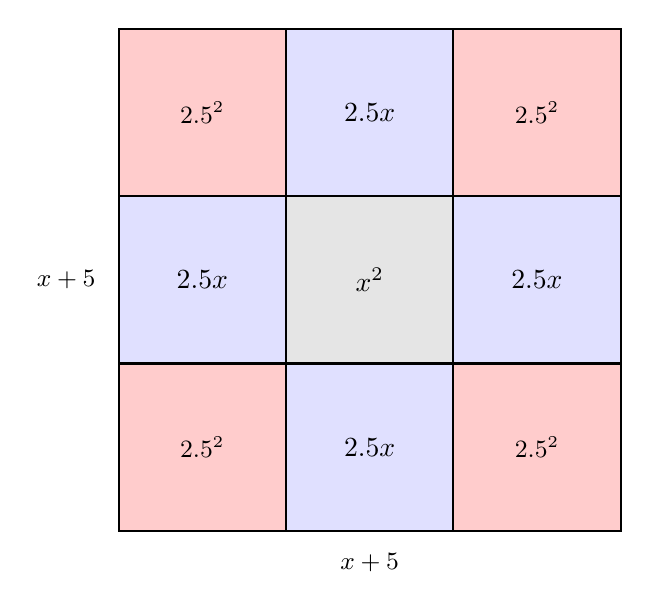
\begin{tikzpicture}[scale=0.85]
			% central square
			\draw[thick,fill=gray!20] (2.5,2.5) rectangle (5,5);
			\node at (3.75,3.75) {$x^2$};
			% four rectangles
			\draw[thick,fill=blue!12] (0,2.5) rectangle (2.5,5);   % left
			\draw[thick,fill=blue!12] (5,2.5) rectangle (7.5,5);   % right
			\draw[thick,fill=blue!12] (2.5,0) rectangle (5,2.5);   % bottom
			\draw[thick,fill=blue!12] (2.5,5) rectangle (5,7.5);   % top
			\node at (1.25,3.75) {$2.5x$};
			\node at (6.25,3.75) {$2.5x$};
			\node at (3.75,1.25) {$2.5x$};
			\node at (3.75,6.25) {$2.5x$};
			% corner squares
			\draw[thick,fill=red!20] (0,0) rectangle (2.5,2.5);
			\draw[thick,fill=red!20] (5,0) rectangle (7.5,2.5);
			\draw[thick,fill=red!20] (0,5) rectangle (2.5,7.5);
			\draw[thick,fill=red!20] (5,5) rectangle (7.5,7.5);
			\node at (1.25,1.25) {\small $2.5^2$};
			\node at (6.25,1.25) {\small $2.5^2$};
			\node at (1.25,6.25) {\small $2.5^2$};
			\node at (6.25,6.25) {\small $2.5^2$};
			% labels
			\node[below] at (3.75,-0.2) {\small $x + 5$};
			\node[left] at (-0.2,3.75) {\small $x+5$};
		\end{tikzpicture}
	\end{center}
	
	The four \emph{missing corner squares} each have side $2.5$, hence area $2.5^2 = 6.25$. Total area to add:
	\[
	4\cdot 6.25 = 25.
	\]
	Adding this to both sides of $x^2 + 10x = 39$:
	\[
	x^2 + 10x + 25 = 39 + 25 = 64.
	\]
	The left side is the area of the completed square of side $x + 5$:
	\[
	(x+5)^2 = 64 \implies x + 5 = 8 \implies x = 3.
	\]
	(Lengths are positive, so we take the positive square root.)
	
	\subsection*{(b) Quadratic formula}
	\[
	x^2 + 10x - 39 = 0 \implies x = \frac{-10 \pm \sqrt{100 + 156}}{2} = \frac{-10 \pm \sqrt{256}}{2} = \frac{-10 \pm 16}{2}.
	\]
	Thus
	\[
	x_1 = \frac{6}{2} = 3,\qquad x_2 = \frac{-26}{2} = -13.
	\]
	
	\subsection*{(c) Average and product}
	Sum of roots $= -10$, product $= -39$. Average:
	\[
	\bar{x} = \frac{3 + (-13)}{2} = -5.
	\]
	Write the roots as $\bar{x} \pm d = -5 \pm d$. Their product is
	\[
	(-5+d)(-5-d) = 25 - d^2 = -39 \implies d^2 = 64 \implies d = 8.
	\]
	Hence the roots are $-5 + 8 = 3$ and $-5 - 8 = -13$.
	
	\subsection*{(d) Comparison}
	All three methods agree: roots $3$ and $-13$.
	
	\begin{itemize}
		\item \textbf{Geometry} yields only $x = 3$ because it interprets $x$ as a \emph{length}; the completed square has side $x+5 = 8 > 0$, and a negative side length is meaningless. The construction automatically discards $x = -13$ (which would give side $x + 5 = -8$, impossible for a geometric square).
		\item \textbf{Verification:}
		\[
		3^2 + 10\cdot 3 = 9 + 30 = 39 \;\checkmark,\qquad
		(-13)^2 + 10(-13) = 169 - 130 = 39 \;\checkmark.
		\]
	\end{itemize}
	The geometric method is a \emph{restricted} solution method (positive roots only); the algebraic methods recover the full solution set over $\mathbb{R}$.
	
	%==========================================================
	\section*{Optional challenge: A geometric identity}
	
	\noindent Let $a > b > 0$. We prove
	\[
	ab = \left(\frac{a+b}{2}\right)^2 - \left(\frac{a-b}{2}\right)^2.
	\]
	
	\noindent\textbf{Setup.} Let $s = \frac{a+b}{2}$ (the average) and $t = \frac{a-b}{2}$ (the half-difference). Consider the square of side $s$. Inside it, place the square of side $t$ in the top-right corner. The \emph{gnomon} is the L-shaped region that remains:
	\[
	\text{Area of gnomon} = s^2 - t^2 = \left(\frac{a+b}{2}\right)^2 - \left(\frac{a-b}{2}\right)^2.
	\]
	
	\begin{center}
		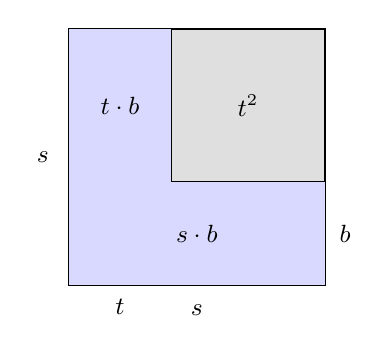
\begin{tikzpicture}[scale=1.3]
			% Outer square side s
			\draw[thick] (0,0) rectangle (2.5,2.5);
			% Inner square side t in top-right corner
			\draw[thick,fill=gray!25] (1.0,1.0) rectangle (2.5,2.5);
			\node at (1.75,1.75) {\small $t^2$};
			% Gnomon shading (L-shape): bottom strip + left strip
			\fill[blue!15] (0,0) rectangle (2.5,1.0); % bottom strip, height s-t = b
			\fill[blue!15] (0,1.0) rectangle (1.0,2.5); % left strip, width t
			\node at (1.25,0.5) {\small $s \cdot b$};
			\node at (0.5,1.75) {\small $t \cdot b$};
			% Labels
			\node[below] at (1.25,-0.1) {\small $s$};
			\node[left] at (-0.1,1.25) {\small $s$};
			% Dimension labels for the two rectangles of the gnomon
			\node[right] at (2.55,0.5) {\small $b$};
			\node[below] at (0.5,-0.05) {\small $t$};
		\end{tikzpicture}
	\end{center}
	
	\noindent\textbf{Why the gnomon has area $ab$.} The gnomon can be split into two non-overlapping rectangles:
	\begin{enumerate}
		\item A bottom rectangle of width $s$ and height $s - t = b$. Its area is $s \cdot b$.
		\item A left rectangle of width $t$ and height $s - t = b$. Its area is $t \cdot b$.
	\end{enumerate}
	Together, their total area is
	\[
	s \cdot b + t \cdot b = (s + t) \cdot b.
	\]
	But recall our definitions: $s = \frac{a+b}{2}$ and $t = \frac{a-b}{2}$. Their sum is exactly $a$:
	\[
	s + t = \frac{a+b}{2} + \frac{a-b}{2} = \frac{2a}{2} = a.
	\]
	Therefore, the total area of the gnomon is $a \cdot b = ab$.
	
	\noindent\textbf{Conclusion.} The same gnomon has area $s^2 - t^2$ (as outer square minus inner square) and area $ab$ (as the two rectangles). Hence
	\[
	ab = \left(\frac{a+b}{2}\right)^2 - \left(\frac{a-b}{2}\right)^2. \qed
	\]
	
	\noindent\textbf{Interpretation.} The identity says: \emph{product = (average)$^2$ $-$ (half-difference)$^2$}. Equivalently, the product is the square of the average diminished by the square of the half-difference. This is exactly the mechanism behind part 5(c): given the average $\bar{x}$ and product $P$, the half-difference $d$ satisfies
	\[
	P = \bar{x}^2 - d^2 \implies d = \sqrt{\bar{x}^2 - P},
	\]
	and the roots are $\bar{x} \pm d$. The gnomon identity is the geometric form of ``sum-and-product determines the roots.''
	
\end{document}